\documentclass{report}
\usepackage[vmargin=2.5cm,hmargin=2.5cm]{geometry}
\usepackage[pdftex]{graphicx}
\usepackage{amsmath}
\newcommand{\HRule}{\rule{\linewidth}{0.5mm}}
\newcommand{\dsum}{\displaystyle\sum}
\def\thesection{\arabic{section}}
\begin{document}
\begin{titlepage}

\begin{center}


% Upper part of the page

\includegraphics[width=0.15\textwidth]{./logo}\\[1cm]    

\textsc{\LARGE Simon Fraser University}\\[1.5cm]

\textsc{\Large CMPT 300: Project II}\\[0.5cm]


% Title
\HRule \\[0.4cm]
%{ \huge \bfseries Project II }\\[0.4cm]
{ \huge \bfseries Design and Implementation of a Monitor Construct. }\\[0.4cm]

\HRule \\[1.5cm]
{ \large \bfseries \emph{Authors}}\\[1cm]

% Author and supervisor
\begin{minipage}{0.26\textwidth}
%\begin{centering}
\begin{flushleft} \large
Joel Fox\\
joelsemail@sfu.ca\\
555555555
\end{flushleft}
\end{minipage}
\begin{minipage}{0.26\textwidth}
\centering
\large
Matt Grandy\\
mattsemail@sfu.ca\\
666666666
\end{minipage}
\begin{minipage}{0.26\textwidth}
\begin{flushright} \large
Andrew Inwood\\
ami2@sfu.ca\\
301020970
\end{flushright}
\end{minipage}

\vfill

% Bottom of the page
{\large \today}

\end{center}

\end{titlepage}

\section{Introduction}
Monitors are a powerful technique for providing mutual exclusion to shared
resources in a multiprogramming environment, because of their ability to simplify the
programming interface for users of the shared resource. They are, however, a complex
construct that must be supported by the compiler for the language that makes use of them.
Seeing as the design goals of C/C++ are primarily based on speed and efficiency of the
resulting code, Monitors are not supported in these languages. 

In this report we design and implement a software interface that simulates the interface
of a Monitor, using the pthreads package to provide the mutual exclusion required. We then
use the Monitor construct to provide mutual exclusion to a hard drive simulator, which receives IO requests 
from multiple users.

\section{High-level Design} %Joel

\section{Analysis} %Andrew
\subsection{Time to Service a Request}
One of the most important metrics in analyzing the performance of the hard drive is the
time it takes after an IO request is made before it is serviced by the hard drive. This
interval is expected to depend on the number of unserviced requests made to the hard drive
thus far, because the servicing thread always has to scan the entire list of requests in
order to find the next request according to the scheduling rule. The way we ensure that
more requests are pushed into the queue is by increasing the number of requesting threads.

In figures
\ref{fig:waittimeElevator} and \ref{fig:waittimeSSTF}, this delay interval is shown as a 
function of the number of request threads for the Elevator and SSTF scheduling algorithms,
respectively.
This data was gathered from running the simulation multiple times, with increasingly many
request threads, and on input data of 1000 requests generated randomly on the disk.
IO requests from anywhere on the disk. 

\begin{figure}
    \centering
    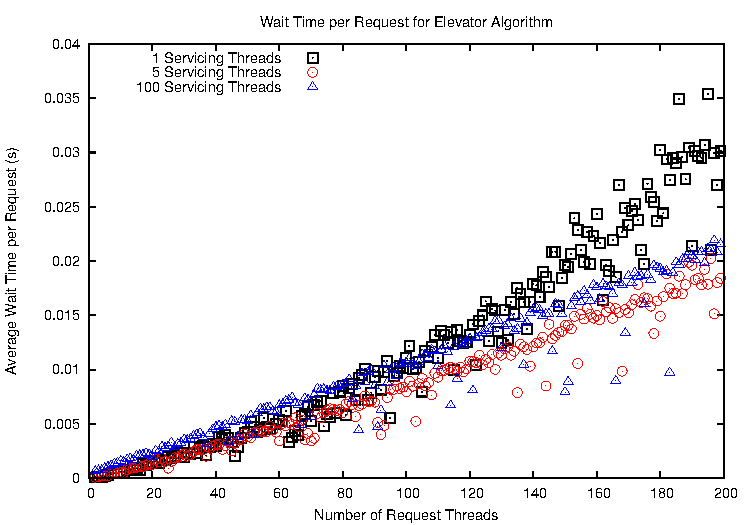
\includegraphics[scale=1]{waittimeElevator.pdf}
    \label{fig:waittimeElevator}
    \caption{The wait time per request is improved by using more than one servicing thread.}
\end{figure}

\begin{figure}
    \centering
    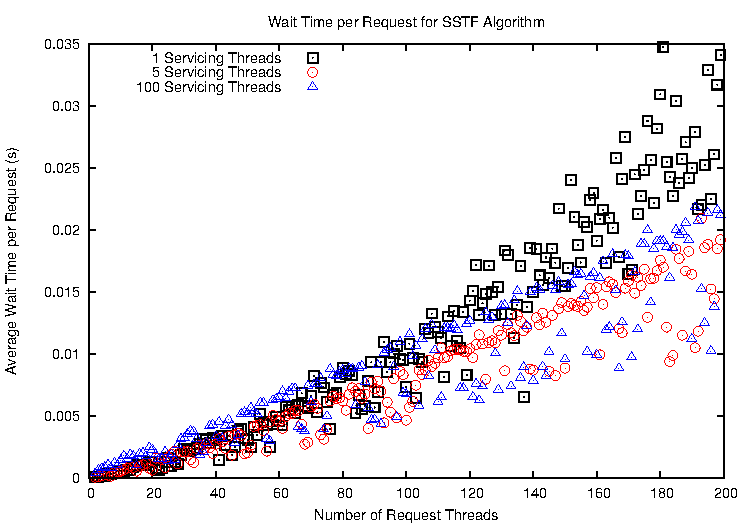
\includegraphics[scale=1]{waittimeSSTF.pdf}
    \label{fig:waittimeSSTF}
    \caption{The wait time per request is improved by using more than one servicing thread.}
\end{figure}
From the graphs, we can make a few observations. Firstly, we can see that the performance
of both algorithms are comparable using this metric, on this input data. This happens because
the behaviour of the two algorithms are similar when the request queue
contains data from everywhere on the disk. In this situation, both algorithms will scan up
and down the disk in succession, servicing requests along the way. 

Secondly, we can note
the change in performance when increasing number of servicing threads are employed. By
increasing from one to five threads, there is a clear improvement in  performance,
especially when there are many request threads. With only one servicing thread,
there is a divergence from linear behaviour, but this divergence is delayed when using a
large number of servicing threads. However, we can see that when using 100 threads, the
performance is reduced from when using 5 threads. This is caused by the overhead of
the system having to maintain a large number of threads. Therefore, performance by this
metric is optimized by using a small number of servicing threads, but more than one.

%This data was generated by running the simulation with increasingly large number of
%requesting threads, since this causes more requests to get onto the queue before the
%servicing thread can service them. Whenever a request was serviced, the wait time and
%number of requests were recorded, and an average was computed for each number of
%requesting threads. From the figure it's clear that the performance of the two algorithms
%are comparable for this input. This happens because when the request queue becomes filled
%with requests from all over the disk, the Elevator and SSTF algorithms behave more or less
%in the same way, scanning forward and backward through the disk in a cycle.
%
There is a test case in which SSTF performs much worse than the Elevator algorithm. The
SSTF algorithm can suffer from starvation when most of the IO requests are on one end of
the disk (say the outer edge), and then a small number of requests are made for the other
end of the disk (inner edge). If
requests for the outer edge keep coming in before the servicing thread has the chance to
clear the queue of requests, then those requests will never run. The elevator algorithm
does not suffer from this problem, of course, since it scans the disk back and forth.
Unfortunately (or perhaps fortunately!) it is very difficult to construct a test case that demonstrates this
behaviour; the scheduling environment makes it difficult to predict how many
requests will be pending at any time, so it is not possible to predict how long the servicing
thread will execute before pthreads forces it to yield.

\subsection{Distance per Request}
In the on the time to service a request, the analysis assumed that all jobs took the same
amount of time to execute, and so the time was mostly attributable to the scheduling
algorithm, and the relative amount of time spent in requesting threads versus the
servicing thread. In real hardware, the IO head will require some time to move to the
desired track, and so this might be a useful metric. Specifically, we measure the average
number of tracks traversed between the time a request is made, and the same request is
serviced. In figures \ref{fig:distanceElevator} and \ref{fig:distanceSSTF} we show this 
quantity with respect to the number of request threads in the simulation, for the
Elevator and SSTF algorithms, respectively.
\begin{figure}
    \centering
    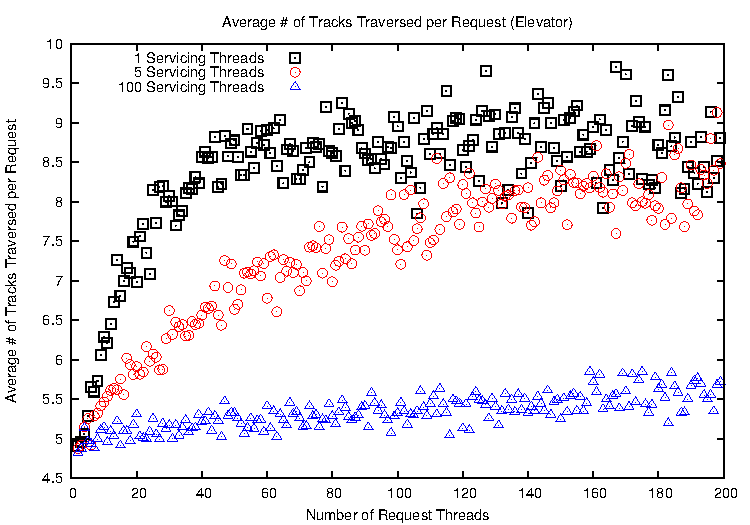
\includegraphics[scale=1]{distanceElevator.pdf}
    \label{fig:distanceElevator}
    \caption{The average number of tracks traversed by the IO head per request can depend
    significantly on the number of servicing threads in use.}
\end{figure}

\begin{figure}
    \centering
    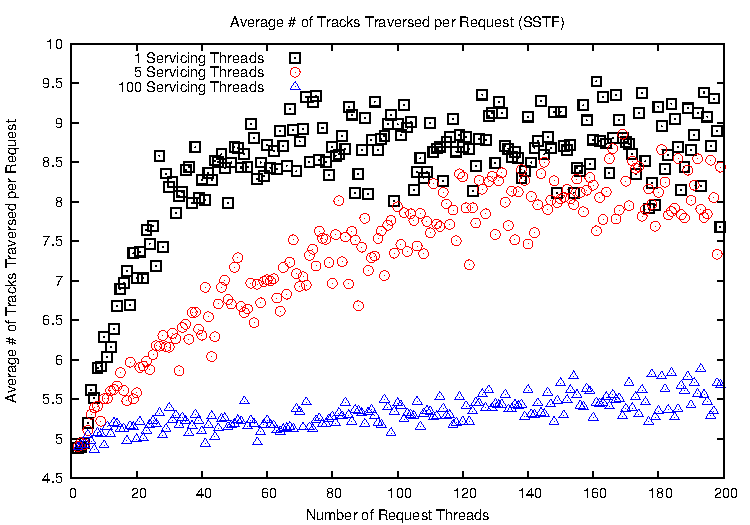
\includegraphics[scale=1]{distanceSSTF.pdf}
    \label{fig:distanceSSTF}
    \caption{Performans of SSTF under the distance metric is comparable to Elevator on
    random input data.}
\end{figure}

Again, it's clear that the two algorithms have similar performance under this metric. This
is again attributable to the behaviour of the two algorithms being similar on the input.
Of particular interest, however, is the profile of the data. When the number of request
threads is fewer than about twenty, the average distance per request increases linearly.
This happens when there are relatively few requests on the queue
(the result of fewer request threads), since the IO head will not travel in a straight line to
the requested track under SSTF or Elevator, but rather will go back and forth between
close requests in SSTF, or in the wrong direction with Elevator. However, when there are
many requests, as explained before, both algorithms will scan the entire disk up and down
servicing all requests. When multiple servicing queues are used, the average distance 
levels off at increasingly
small values. This happens because having more servicing threads reduces the number of
pending requests at any time, and so the average distance travelled does not grow as
much.

Note that regardless of the number of servicing threads, the average number of tracks
traversed begins at around 5. This is the result of our input data being random, and it
can be shown that the expected distance travelled is 5 when using a hard drive of size 15,
as we do in our simulations. When there is only 1 request thread, each request is usually
serviced immediately because the act of requesting when there are no requests pending
signals the servicing thread to do some work. Since the requests are designed to be
random, the average distance ($D$) travelled is the average distance between any two
tracks. This is computed below.
\begin{align*}
\mathrm{E}(D) &= \dsum_{i=0}^N D\times\mathrm{P}(D),\text{expectation formula}\\
              &= \frac{N}{N^2} + \dsum_{i=1}^N (N - i)\times \frac{2i}{N^2},\text{$N$ ways for
                                                      positions to be identical} \\
              &= \frac{1}{N^2}\left[ 2N\cdot\frac{N\cdot(N+1)}{2} 
              - 2\cdot\left(\frac{1}{6}\cdot N \cdot (N+1) \cdot (2N + 1) \right)
              + N \right], \text{using summation formulae}\\
              &= N+1 - \frac{(N+1)\cdot(2N + 1)}{3N} + \frac{1}{N}.
\end{align*}
Plugging in $N = 15$ yields E($D$) = 5.04, which is close to the observed value.
%
%As an example, if there are only two requests
%on the queue, both algorithms will cause the IO head to travel directly to the requested
%track; however, if there are a few more requests, then the Elevator algorithm may travel
%in the opposite direction before coming back, and SSTF might go back and forth serving the
%nearest requests before it gets to the last one. Once the number of requests gets to be large 
%(caused by more request threads), both
%algorithms will service requests linearly on the disk, making a straight path to each
%request, which is why the distance levels off and even decreases slightly with increasing
%number of request threads.
%
%%As a point of interest, in figure \ref{fig:distance100}, we show the same data but now
%%taken when there are 100 servicing threads active. Here we no longer see the levelling off
%%effect, because the servicing threads are more effective at keeping the number of pending
%%requests low.
%This data shows us that there is a peak in distance that we would like to avoid, either by
%using sufficiently few request threads, or sufficiently many. The exact number would need
%to be found experimentally for the expected input.
%
\subsection{Reversals per Request}
Another hardware consideration is the number of times the IO head will need to switch
directions after a request is made and before it is serviced. Just like the distance
metric, in real hardware it is expected that instructing the IO head to reverse direction
would take some time, and it may be a desirable quantity to minimize. Figures
\ref{fig:turnsElevator} and \ref{fig:turnsSSTF} show this quantity with respect to the 
number of request threads, for the Elevator and SSTF algorithms, respectively.
\begin{figure}
    \centering
    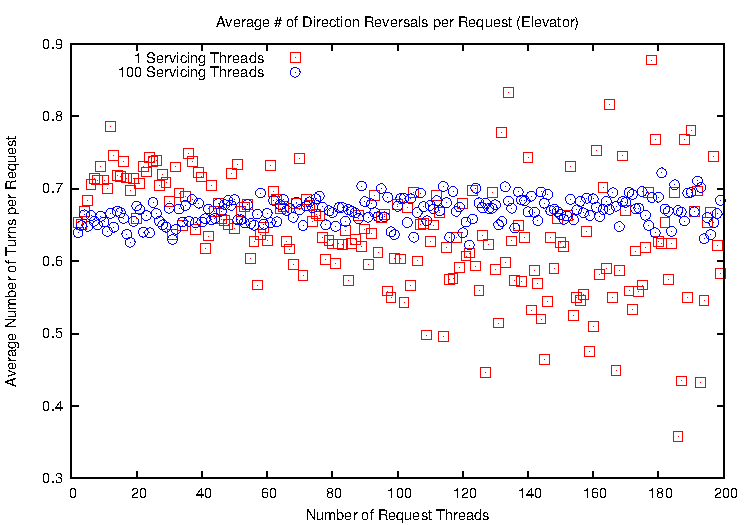
\includegraphics[scale=1]{turnsElevator.pdf}
    \label{fig:turnsElevator}
    \caption{Due to the nature of the Elevator algorithm, the number of turns per request
    is guaranteed never to be more than one.}
\end{figure}

\begin{figure}
    \centering
    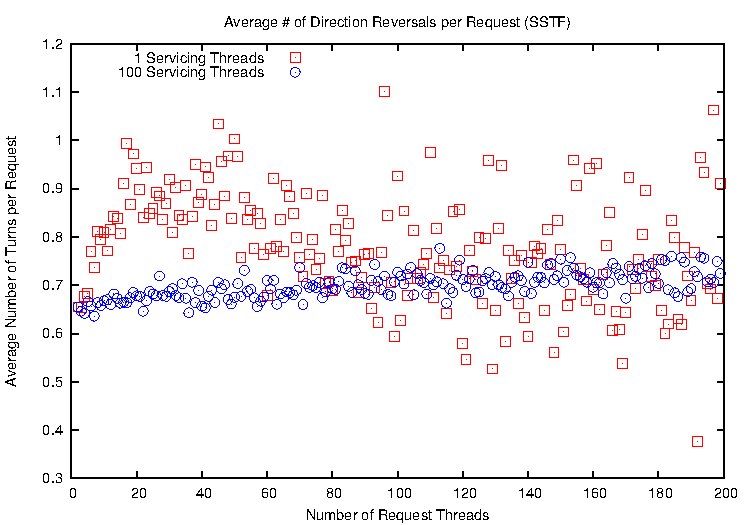
\includegraphics[scale=1]{turnsSSTF.pdf}
    \label{fig:turnsSSTF}
    \caption{The number of reversals when using SSTF can be more than one per request.}
\end{figure}

For both algorithms, there is an initial increase in the number of reversals as the number
of request threads increase. This again is attributable to a non-empty request queue which
is sparse. This initial increase is lost when the number of servicing threads is
increased, because the number of pending requests is kept very low.

This is the first metric for which there is a measurable difference in performance. When
there is only one request thread, the SSFT algorithm had runs whose \emph{average} number
of reversals was greater than one. This means that IO head had to reverse direction on
almost every request, and sometimes more than once. This is definitely not very good
behaviour if reverals want to be kept to a minimum. In comparison, the number of reversals
for the Elevator don't vary as much, and the average number of reverals rarely were more
than 0.8.

%The data shows that the two algorithms perform comparably on this input, and have a
%profile similar to that of the distance metric (although on a smaller scale). The
%explanation for this behaviour is the same as that for the distance metric behaviour: when
%there are few requests on the queue, both algorithms may make a detour 
\section{Listings} %will contain trial runs and source code


\tableofcontents %automatically generated
\end{document}
